\begin{frame}{Winners ImageNet Large Scale Visual Recognition Challenge}
  \begin{figure}
    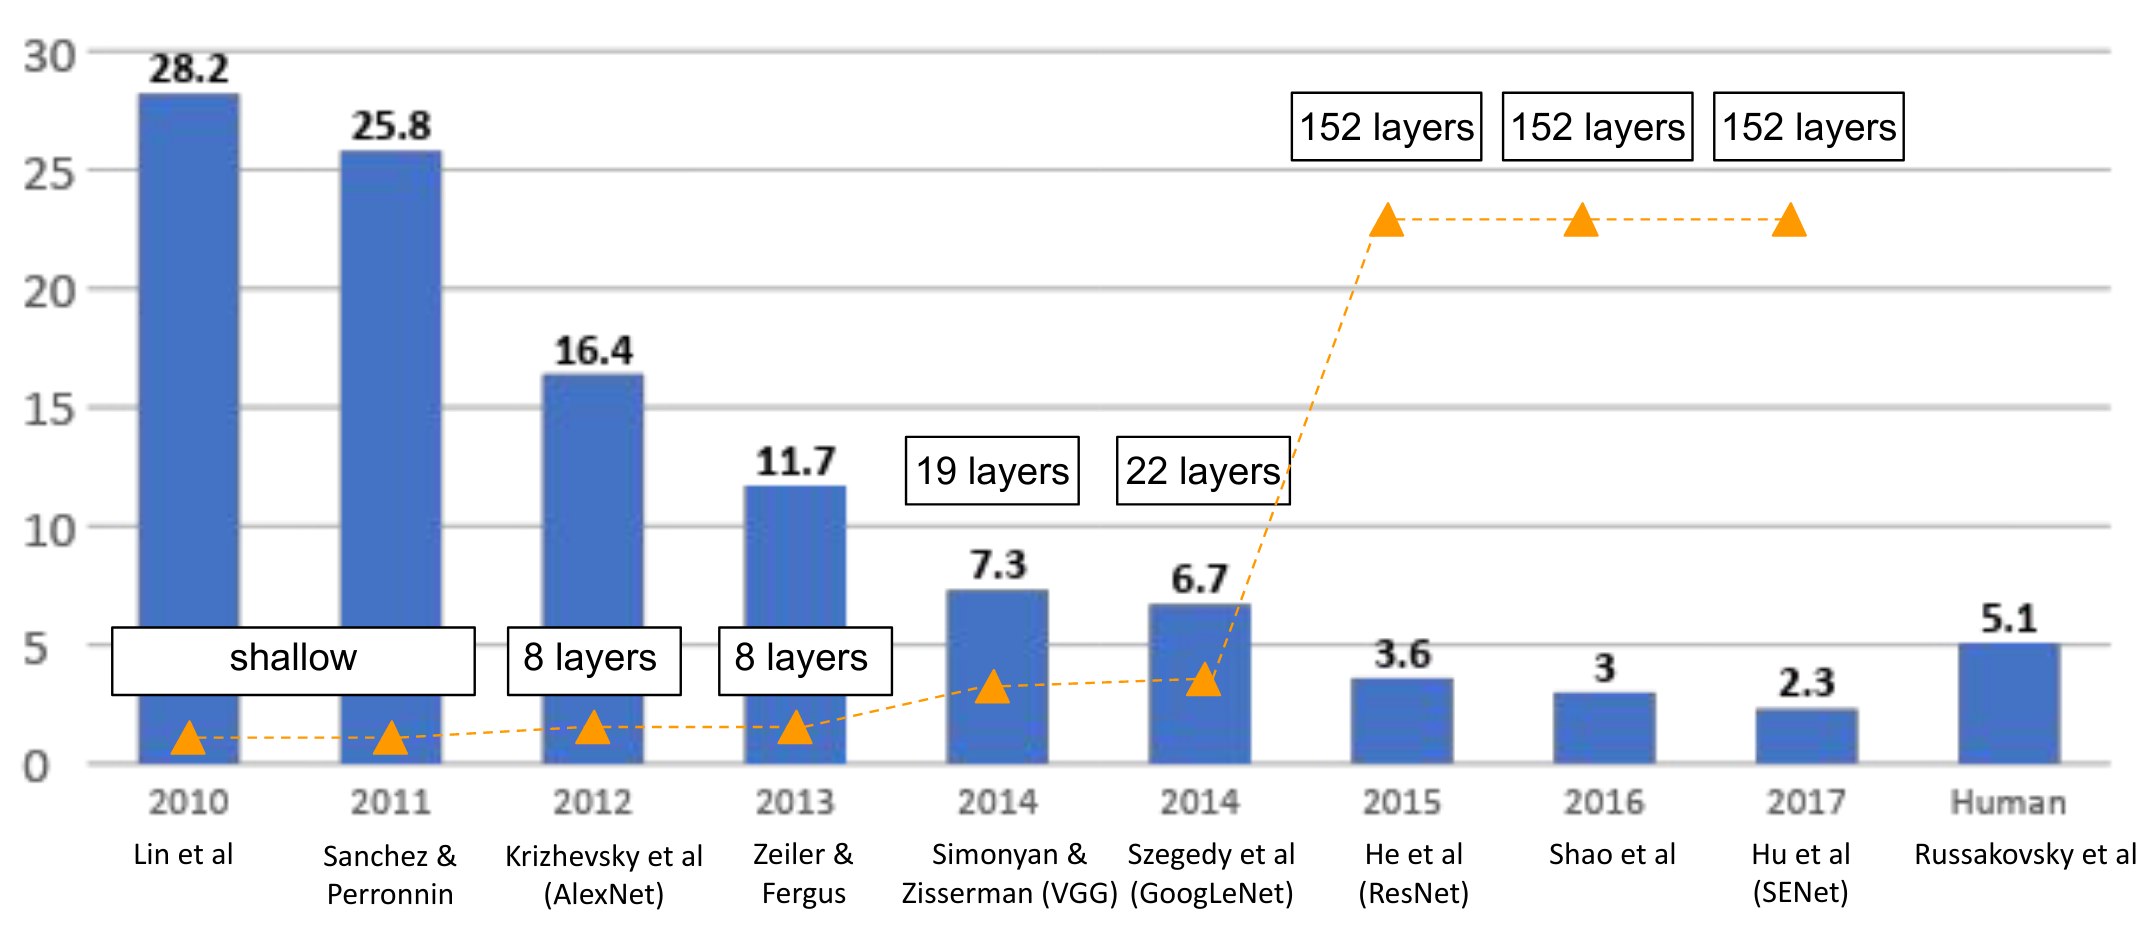
\includegraphics[width=0.9\textwidth]{winners}
  \end{figure}

  \note{
    \begin{itemize}
      \item Image from Stanford CS231n Lecture 9, Fei-Fei Li \url{http://cs231n.stanford.edu/slides/2021/lecture_9.pdf}
    \end{itemize}
  }
\end{frame}


\begin{frame}{Accuracy ImageNet Ops/Params}
  \begin{figure}
    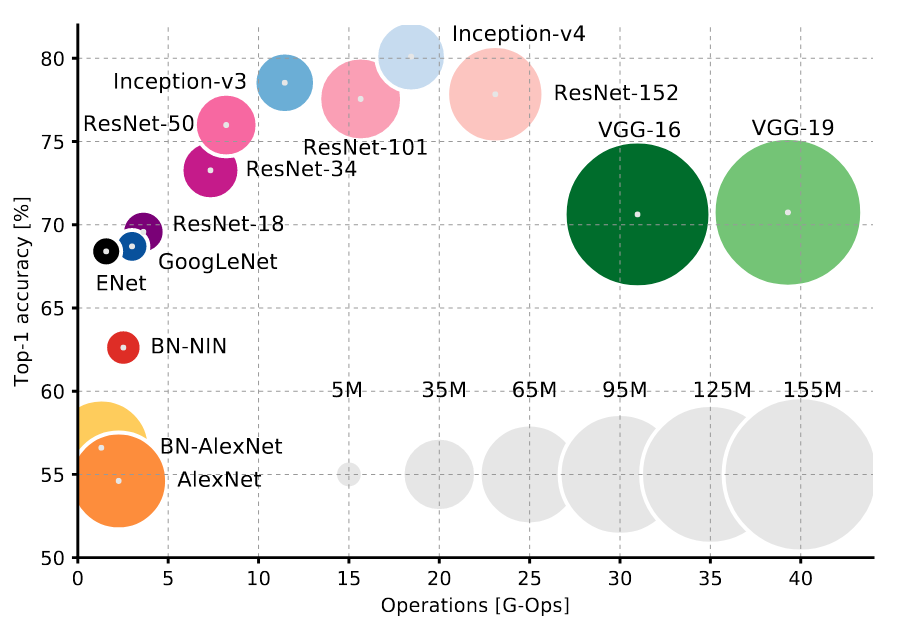
\includegraphics[width=0.7\textwidth]{accuracy_imagenet_params_flops}
  \end{figure}

  \note{
    \begin{itemize}
      \item Image from An Analysis of Deep Neural Network Models for Practical Applications, Canziani et al, 2017
    \end{itemize}
  }
\end{frame}


\begin{frame}{Efficiency}
  \begin{figure}
    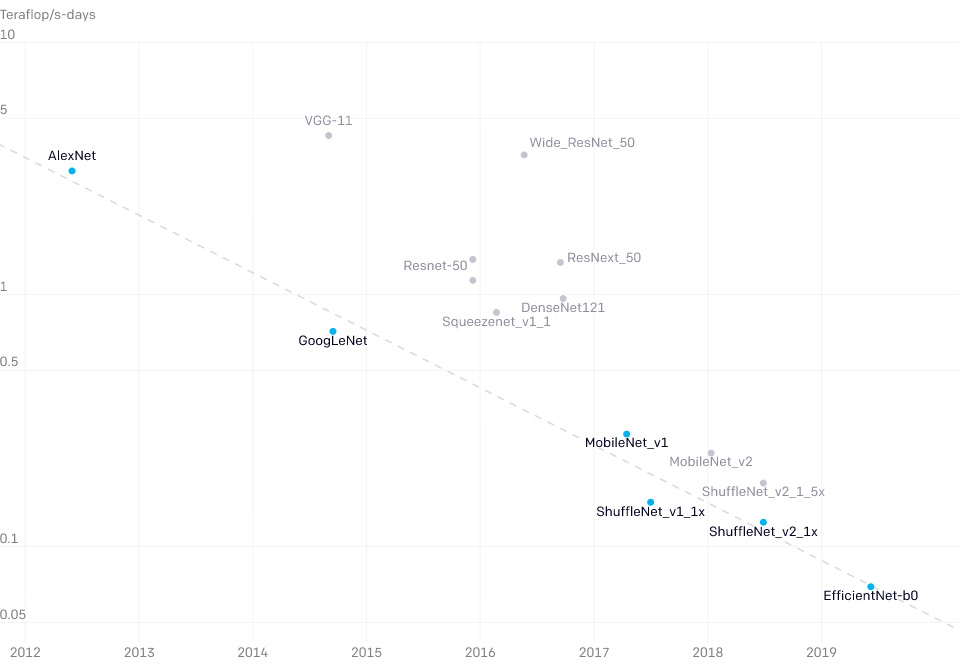
\includegraphics[width=0.8\textwidth]{efficiency}
  \end{figure}

  \note{
    \begin{itemize}
      \item Total amount of compute in teraflops/s-days used to train to AlexNet level performance. Lowest compute points at any given time shown in blue, all points measured shown in gray.
      \item Image from \url{https://openai.com/blog/ai-and-efficiency/}
    \end{itemize}
  }
\end{frame}
